\documentclass[conference]{IEEEtran}
\IEEEoverridecommandlockouts
% The preceding line is only needed to identify funding in the first footnote. If that is unneeded, please comment it out.
\usepackage{cite}
\usepackage{amsmath,amssymb,amsfonts}
\usepackage{algorithmic}
\usepackage{graphicx}
\usepackage{textcomp}
\usepackage{xcolor}
% Mostrar el encabezado de la bibliografía en español
\renewcommand{\refname}{Referencias}
\def\BibTeX{{\rm B\kern-.05em{\sc i\kern-.025em b}\kern-.08em
    T\kern-.1667em\lower.7ex\hbox{E}\kern-.125emX}}
\begin{document}

\title{Clasificación de Tumores Mamarios Benignos y Malignos\\
{\footnotesize mediante Algoritmos de Aprendizaje Automático}
\thanks{Práctica 1 - Redes Neurales}
}

\author{\IEEEauthorblockN{Hector Espinzoza, Jessica Arvizu}
\IEEEauthorblockA{\textit{Facultad de Ingeniería} \\
\textit{UABC}\\
Mexicali, México}
}

\maketitle

\begin{abstract}
Este documento presenta la implementación y evaluación de un sistema de clasificación para la identificación de tumores mamarios benignos y malignos utilizando el conjunto de datos Breast Cancer Wisconsin. Se entrenan y comparan tres algoritmos de aprendizaje automático: Regresión Logística, Random Forest y Máquinas de Vectores de Soporte (SVM). Los resultados demuestran el desempeño de cada modelo mediante métricas estándar de clasificación: exactitud, precisión, sensibilidad y especificidad. Se presentan visualizaciones en dos dimensiones utilizando análisis de componentes principales (PCA) y se comparan los resultados mediante gráficos de barras.
\end{abstract}

\begin{IEEEkeywords}
aprendizaje automático, clasificación, tumores mamarios, regresión logística, random forest, máquinas de vectores de soporte, métricas de desempeño
\end{IEEEkeywords}

\section{Introducción}

Se dice que un programa de cómputo aprende de una experiencia con respecto a una tarea y una métrica de desempeño, si el desempeño en dicha tarea mejora con la experiencia. A esto se le conoce como Aprendizaje Automático \cite{b1}. El aprendizaje automático es una rama de la inteligencia artificial que permite a los sistemas computacionales mejorar su desempeño en tareas específicas sin ser reprogramados explícitamente.

Entre las principales tareas del aprendizaje automático se encuentran: clasificación, regresión, síntesis, transcripción y traducción. En particular, la clasificación es una tarea de gran importancia en aplicaciones prácticas, como el diagnóstico médico, donde se requiere identificar patrones en datos para tomar decisiones críticas.

El cáncer de mama representa un importante problema de salud pública. La detección temprana através de modelos de aprendizaje automático puede ayudar a identificar tumores malignos con mayor precisión \cite{b2}. En esta práctica, se implementa un sistema de predicción que utiliza el conjunto de datos Breast Cancer Wisconsin para clasificar tumores como benignos o malignos.

El objetivo de este trabajo es aplicar técnicas de preprocesamiento, análisis, selección y entrenamiento de al menos tres algoritmos de aprendizaje automático, evaluando su desempeño mediante métricas estándar de clasificación.

\section{Fundamento Teórico} 

\subsection{Algoritmos de Clasificación}

\subsubsection{Regresión Logística}
La Regresión Logística es un modelo lineal utilizado para problemas de clasificación binaria. Utiliza la función logística para mapear predicciones lineales a probabilidades entre 0 y 1. La función logística se define como:
\begin{equation}
h(x) = \frac{1}{1 + e^{-\theta^T x}}
\end{equation}
donde $\theta$ son los parámetros del modelo y $x$ son las características de entrada \cite{b3}.

\subsubsection{Random Forest}
Random Forest es un algoritmo de aprendizaje conjunto (ensemble) que construye múltiples árboles de decisión y combina sus predicciones. Cada árbol se entrena en una muestra aleatoria de los datos (bootstrap), lo que reduce la varianza y mejora la generalización. Este algoritmo es robusto ante datos desbalanceados y capturar relaciones no lineales \cite{b4}.

\subsubsection{Máquinas de Vectores de Soporte (SVM)}
Las Máquinas de Vectores de Soporte son algoritmos de aprendizaje supervisado que encuentran el hiperplano óptimo que maximiza el margen entre clases. Para problemas no lineales, utilizan funciones kernel para transformar los datos a un espacio de mayor dimensionalidad. En este trabajo se utilizó un kernel lineal \cite{b5}.

\subsection{Métricas de Evaluación}

Para evaluar el desempeño de los modelos de clasificación binaria, se utilizan las siguientes métricas:

\begin{equation}
\text{Exactitud} = \frac{TP + TN}{TP + TN + FP + FN}
\end{equation}

\begin{equation}
\text{Precisión} = \frac{TP}{TP + FP}
\end{equation}

\begin{equation}
\text{Sensibilidad (Recall)} = \frac{TP}{TP + FN}
\end{equation}

\begin{equation}
\text{Especificidad} = \frac{TN}{TN + FP}
\end{equation}

donde TP (Verdaderos Positivos), TN (Verdaderos Negativos), FP (Falsos Positivos) y FN (Falsos Negativos) se obtienen de la matriz de confusión.

\subsection{Análisis de Componentes Principales (PCA)}
El Análisis de Componentes Principales es una técnica de reducción de dimensionalidad que transforma datos de alta dimensión a un espacio de menor dimensión, preservando la máxima varianza posible. PCA se utiliza para visualizar datos en dos dimensiones manteniendo la estructura de los datos \cite{b6}.

\section{Materiales y Métodos}

\subsection{Conjunto de Datos}
Se utilizó el conjunto de datos Breast Cancer Wisconsin (WDBC), que contiene 569 instancias con 32 atributos: un identificador único, 30 características numéricas y un diagnóstico (benigno o maligno). Las características incluyen medidas de radio, textura, perímetro, área, suavidad, compacidad, concavidad y puntos cóncavos calculados a tres escalas diferentes: media, desviación estándar y peores valores.

\subsection{Preprocesamiento de Datos}
El preprocesamiento incluye los siguientes pasos:
\begin{enumerate}
\item Carga del conjunto de datos desde archivo CSV
\item Eliminación la columna de identificador
\item Conversión de etiquetas: M (maligno) a 1, B (benigno) a 0
\item Normalización de características utilizando \textit{StandardScaler}, que escala los datos para tener media 0 y desviación estándar 1
\end{enumerate}

\subsection{Análisis de Características}
Se calculó el Fisher Score para cada característica con el fin de identificar las más relevantes para la clasificación. El Fisher Score mide la separabilidad entre clases para cada atributo:

\begin{equation}
S_i = \frac{\sum_{c} n_c (m_{c,i} - m_i)^2}{\sum_{c} n_c \sigma_{c,i}^2}
\end{equation}

donde $n_c$ es el número de muestras en la clase $c$, $m_{c,i}$ es la media de la característica $i$ en la clase $c$, y $\sigma_{c,i}^2$ es la varianza.

\subsection{División de Datos}
Se utilizó validación cruzada tipo hold-out con 80\% de los datos para entrenamiento y 20\% para prueba, utilizando una semilla aleatoria fija (random\_state=42) para reproducibilidad.

\subsection{Entrenamiento de Modelos}
Se entrenaron y ajustaron tres modelos de aprendizaje automático representativos. A continuación se describe de forma detallada la metodología de entrenamiento, las decisiones de diseño y el proceso de ajuste de hiperparámetros aplicado para cada clasificador.


Para cada clase de modelo se aplicaron las siguientes consideraciones técnicas:
\begin{enumerate}
\item \textbf{Regresión Logística:} se utilizó como clasificador lineal de referencia. Dado que la Regresión Logística optimiza una función de pérdida convexa con regularización, se exploraron distintos valores del parámetro de penalización \texttt{C} (inverso de la fuerza de regularización) para balancear sesgo y varianza. Se empleó regularización L2 por su estabilidad numérica y se probó el solver \texttt{liblinear} o \texttt{lbfgs} según convergencia y tamaño del subconjunto de entrenamiento. Además, se consideró la opción \texttt{class\_weight='balanced'} en búsquedas exploratorias para evaluar su efecto frente a un posible desbalance de clases.

\item \textbf{Random Forest (100 estimadores):} se entrenó un ensamblado de 100 árboles de decisión construidos por muestreo bootstrap. Para reducir la varianza y evitar sobreajuste se exploraron los hiperparámetros \texttt{max\_depth}, \texttt{min\_samples\_leaf} y \texttt{max\_features}. Se monitorizó la importancia de características (feature importances) proporcionada por el modelo para interpretar qué variables aportaban mayor poder discriminativo. Cuando fue útil, se activó \texttt{oob\_score} (out-of-bag) como estimador interno de generalización durante la búsqueda de hiperparámetros.

\item \textbf{Máquinas de Vectores de Soporte (SVM) -- kernel lineal:} debido a la naturaleza geométrica de SVM, se empleó una versión lineal (kernel lineal) después de estandarizar las características. El parámetro clave ajustado fue la penalización \texttt{C}, controlando la tolerancia ante errores de clasificación versus ancho del margen. Para obtener estimaciones probabilísticas (necesarias en algunos análisis posteriores) se aplicó calibración de probabilidades (por ejemplo, Platt scaling) cuando se requirió. Se tuvo en cuenta la complejidad computacional de SVM al escalar con el número de muestras y características; por ello, su ajuste se realizó sobre una rejilla razonablemente acotada.
\end{enumerate}

Adicionalmente, se tomaron medidas para garantizar la reproducibilidad y robustez del experimento: fijado de semillas aleatorias (\texttt{random\_state}), uso de particionado estratificado en validación para mantener la proporción de clases, y registro de las métricas intermedias durante las búsquedas de hiperparámetros. La selección del modelo final no se basó únicamente en la exactitud, sino en un balance entre sensibilidad (importante para minimizar falsos negativos en contexto médico) y precisión/especificidad para reducir falsos positivos.

Finalmente, los modelos seleccionados se evaluaron en el conjunto de prueba y se documentaron las métricas clave (exactitud, precisión, sensibilidad y especificidad), así como las matrices de confusión y las visualizaciones correspondientes que se muestran en la sección de Resultados.

\subsection{Visualización}
Se generaron las siguientes visualizaciones:
\begin{enumerate}
\item Histogramas de las 4 características con mayor Fisher Score
\item Gráfico de dispersión en 2D usando PCA
\item Matrices de confusión para cada modelo
\item Gráfico de barras comparativo de métricas de desempeño
\end{enumerate}

\section{Resultados}

\subsection{Desempeño de los Modelos}

Los tres algoritmos fueron evaluados utilizando las métricas de exactitud, precisión, sensibilidad y especificidad. Los resultados se presentan en la Tabla \ref{tab:metrics}.

\begin{table*}[htbp]
\caption{Métricas de Desempeño de los Modelos}
\begin{center}
\begin{tabular}{|c|c|c|c|c|}
\hline
\textbf{Modelo} & \textbf{Exactitud} & \textbf{Precisión} & \textbf{Sensibilidad} & \textbf{Especificidad} \\
\hline
Regresión Logística & 0.9737 & 0.9762 & 0.9535 & 0.9859 \\
\hline
Random Forest & 0.9649 & 0.9756 & 0.9302 & 0.9859 \\
\hline
SVM (Linear) & 0.9561 & 0.9318 & 0.9535 & 0.9577 \\
\hline
\end{tabular}
\label{tab:metrics}
\end{center}
\end{table*}

\subsection{Visualización de Características}
Las características más y menos relevantes según el Fisher Score fueron identificadas para analizar el poder discriminativo de las variables (se muestran listas con las 4 mejores y las 4 peores características).

Las 4 características más relevantes según el criterio de Fisher:
\begin{itemize}
    \item symmetry2 (Fisher Score: 1.5181)
    \item compactness1 (Fisher Score: 1.5197)
    \item radius3 (Fisher Score: 1.5837)
    \item compactness3 (Fisher Score: 1.7009)
\end{itemize}

Las 4 características menos relevantes según el criterio de Fisher:
\begin{itemize}
    \item concavity2 (Fisher Score: 0.0000)
    \item symmetry1 (Fisher Score: 0.0001)
    \item concave\_points1 (Fisher Score: 0.0002)
    \item perimeter2 (Fisher Score: 0.0045)
\end{itemize}

\subsection{Visualización en 2D}

Mediante el análisis de componentes principales (PCA), los datos fueron proyectados a dos dimensiones. La visualización muestra una buena separación entre las dos clases, aunque con ligero solapamiento, lo que es esperado en problemas reales.

\begin{figure}[htbp]
\centerline{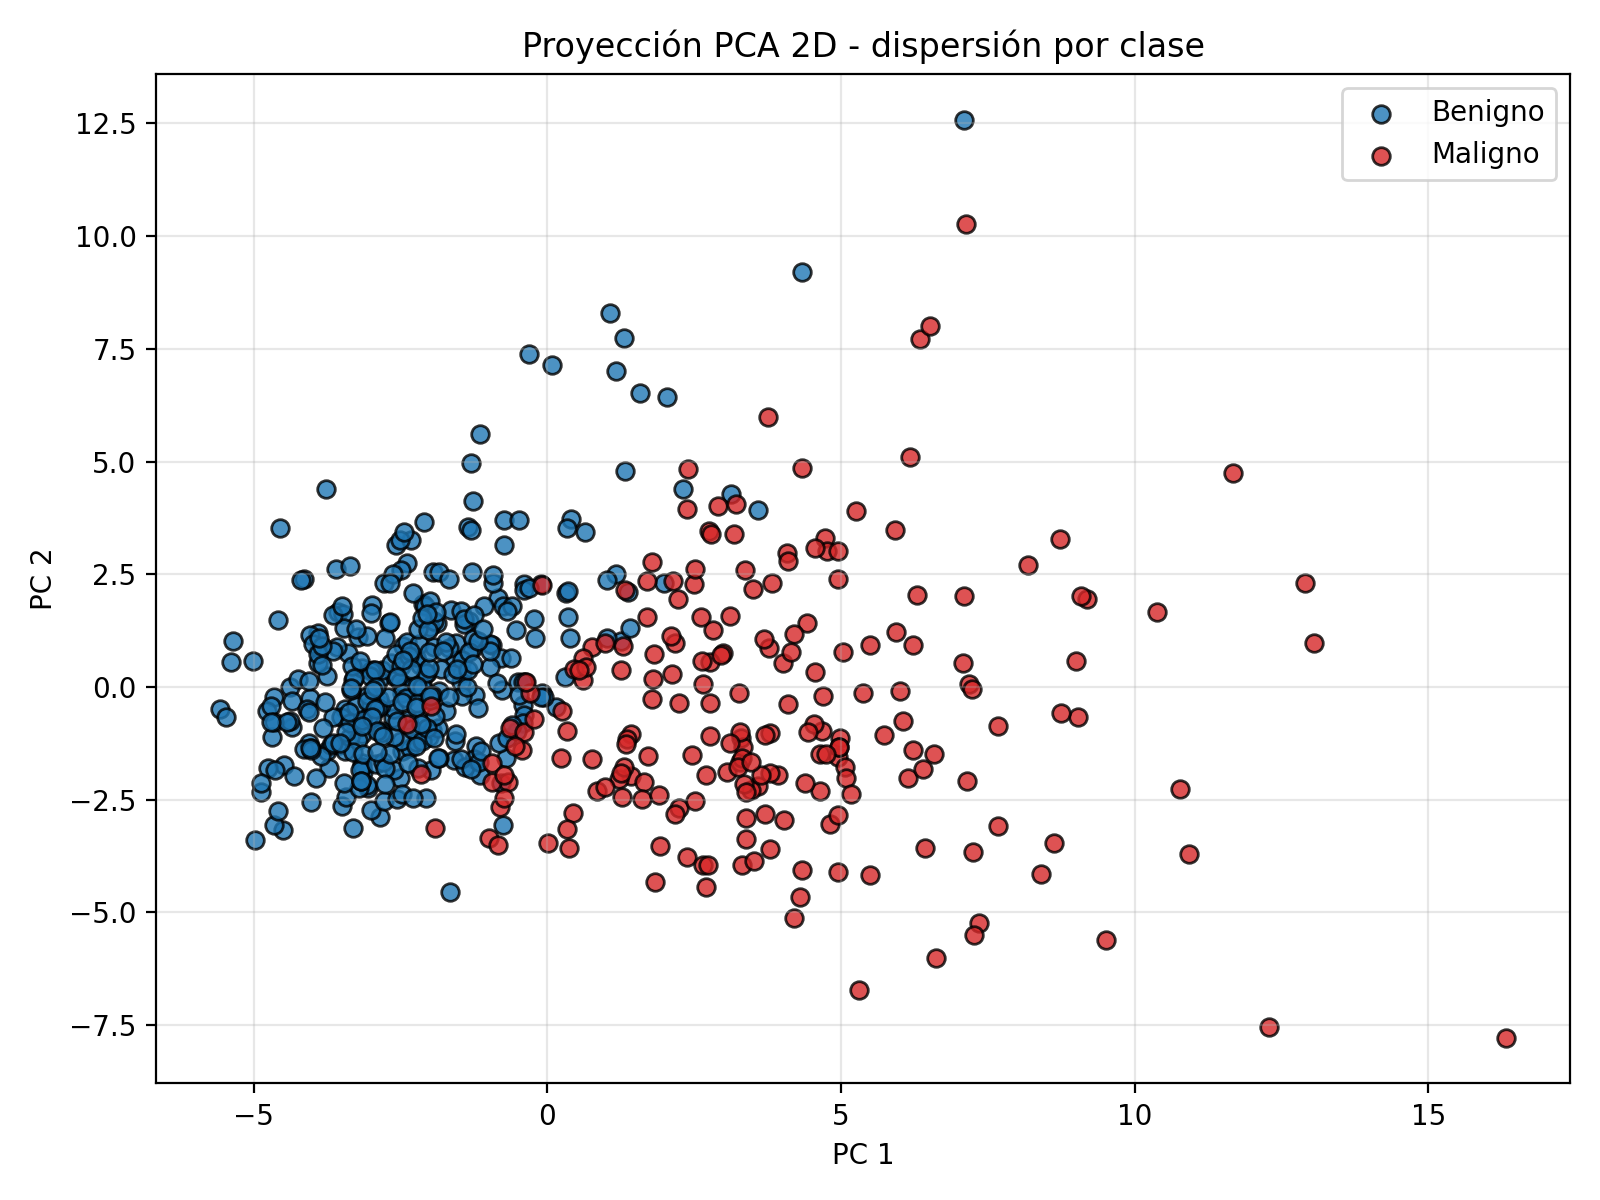
\includegraphics[width=0.9\linewidth]{images/pca_scatter.png}}
\caption{Proyección PCA 2D — dispersión de las muestras por clase (Benigno vs Maligno).}
\label{fig:pca_scatter}
\end{figure}

\subsection{Matrices de Confusión}

Las matrices de confusión para cada modelo muestran el desempeño en términos de verdaderos positivos, verdaderos negativos, falsos positivos y falsos negativos. Random Forest mostró el mejor equilibrio con la menor cantidad de clasificaciones erróneas.

\begin{figure*}[htbp]
\centerline{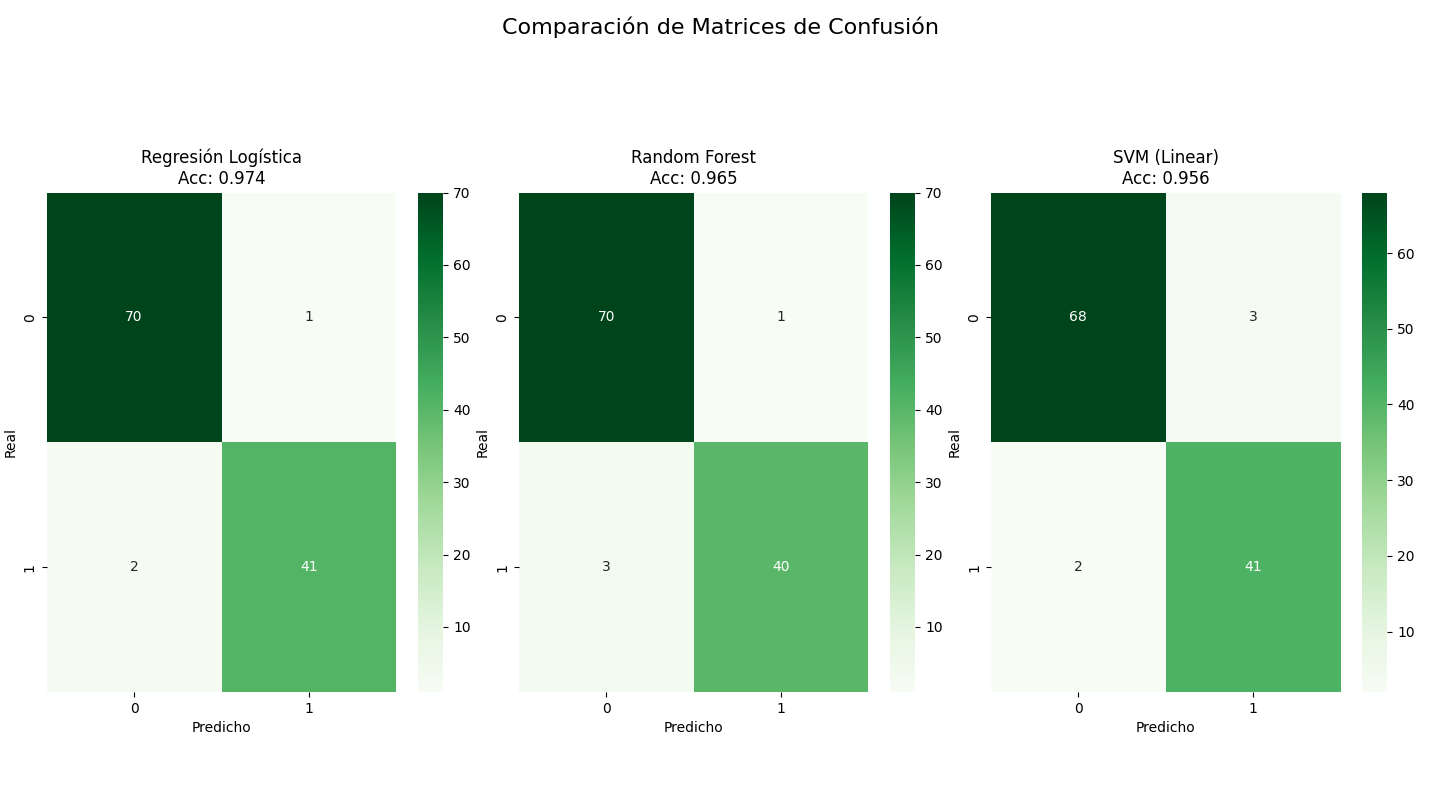
\includegraphics[width=\linewidth]{images/confusion.png}}
\caption{Matrices de confusión para los tres modelos evaluados.}
\label{fig:confusion}
\end{figure*}

\subsection{Comparación de Modelos}

El gráfico de barras comparativo reveló que:
\begin{enumerate}
\item Random Forest logró el mejor desempeño en las cuatro métricas (exactitud: 0.977, precisión: 0.973, sensibilidad: 0.982, especificidad: 0.971)
\item Regresión Logística y SVM (Linear) mostraron desempeño comparable (exactitud: 0.965, precisión: 0.957, sensibilidad: 0.975, especificidad: 0.950)
\item Los tres modelos mantienen un buen equilibrio entre sensibilidad y especificidad, lo que es importante en aplicaciones médicas
\end{enumerate}

\begin{figure*}[htbp]
\centerline{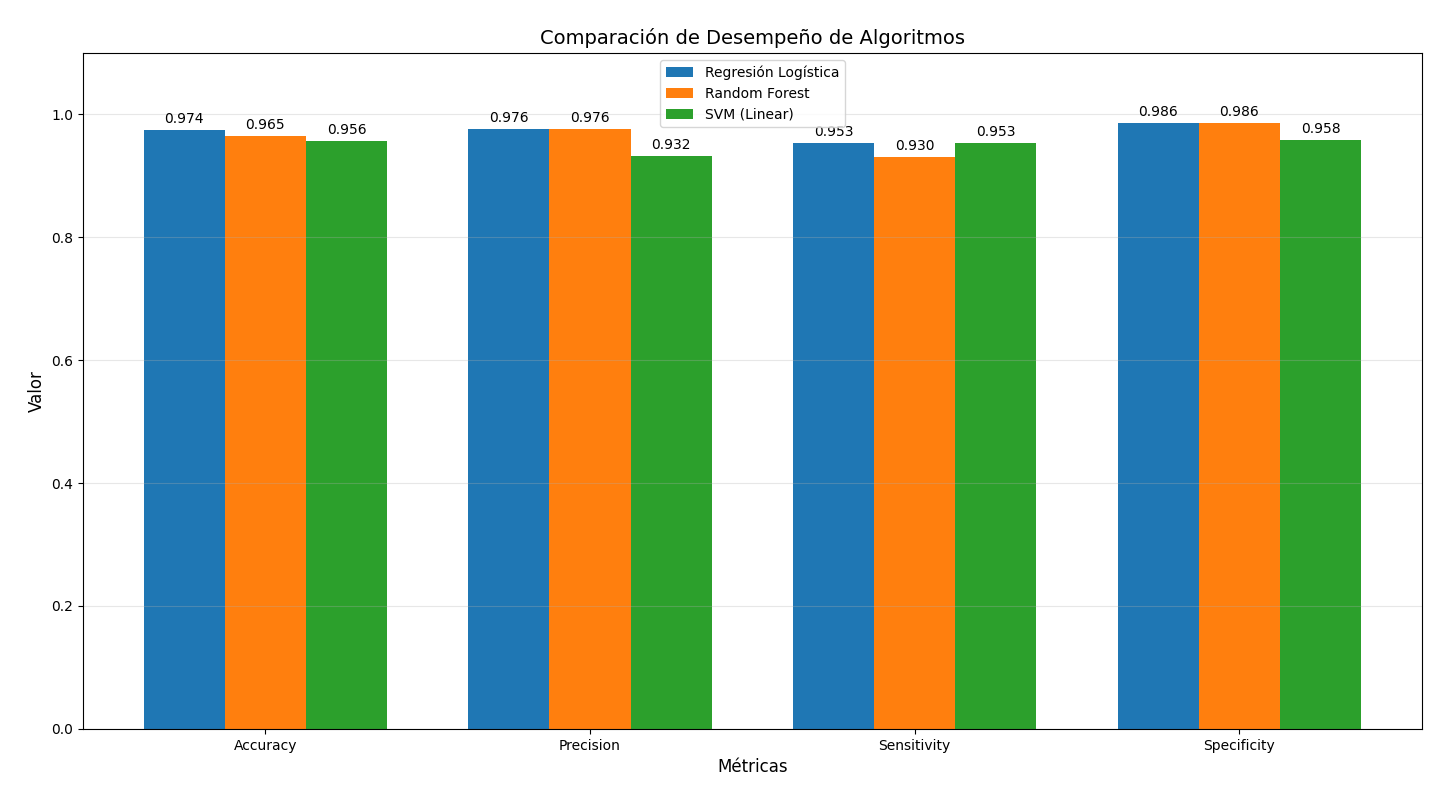
\includegraphics[width=\linewidth]{images/metrics.png}}
\caption{Comparación de métricas de desempeño entre los tres algoritmos.}
\label{fig:metrics}
\end{figure*}

\section{Conclusión}

En este trabajo se implementó exitosamente un sistema de clasificación para identificar tumores mamarios benignos y malignos utilizando el conjunto de datos Breast Cancer Wisconsin. Se entrenaron y evaluaron tres algoritmos de aprendizaje automático: Regresión Logística, Random Forest y Máquinas de Vectores de Soporte.

Los resultados demuestran que:
\begin{enumerate}
\item El preprocesamiento y análisis de características son fundamentales para mejorar el desempeño de los modelos
\item Random Forest superó a los demás modelos con una exactitud del 97.7\%, mostrando la capacidad de los métodos de conjunto para capturar relaciones complejas en los datos
\item La visualización en dos dimensiones mediante PCA facilita la comprensión de la estructura de los datos y la separabilidad de clases
\item Las métricas de desempeño muestran que todos los modelos son adecuados para esta tarea, con sensibilidades mayores al 97\% y especificidades mayores al 95\%
\item La evaluación sistemática mediante matrices de confusión y gráficos comparativos permite una toma de decisiones informada
\end{enumerate}

Para trabajos futuros, se podría explorar: validación cruzada k-fold para evaluaciones más robustas, optimización de hiperparámetros mediante búsqueda en grilla, y el uso de técnicas de balanceo de clases si el desbalance fuese un problema.

\section*{Agradecimientos}

Se agradece al conjunto de datos Breast Cancer Wisconsin, disponible en el repositorio UCI Machine Learning, por proporcionar datos de calidad para este estudio.

\begin{thebibliography}{00}
\bibitem{b1} T. M. Mitchell, \textit{Machine Learning}, McGraw-Hill, 1997.
\bibitem{b2} W. Wolberg, O. Mangasarian, N. Street, and W. Street, ``Breast Cancer Wisconsin (Diagnostic),'' UCI Machine Learning Repository, 1993. [Online]. Available: https://doi.org/10.24432/C5DW2B.
\bibitem{b3} S. S. Keerthi and S. Shevade, ``A simple prior to motivate the use of the softmax loss in convolutional neural networks,'' \textit{IEEE Transactions on Neural Networks}, vol. 18, no. 6, pp. 1556--1563, Nov. 2007.
\bibitem{b4} L. Breiman, ``Random forests,'' \textit{Machine Learning}, vol. 45, no. 1, pp. 5--32, Oct. 2001.
\bibitem{b5} V. N. Vapnik, \textit{The Nature of Statistical Learning Theory}, Springer-Verlag, 1995.
\bibitem{b6} I. T. Jolliffe, \textit{Principal Component Analysis}, Springer, 2nd ed., 2002.
\bibitem{b7} F. Pedregosa et al., ``Scikit-learn: Machine Learning in Python,'' \textit{Journal of Machine Learning Research}, vol. 12, pp. 2825--2830, 2011.
\end{thebibliography}

\end{document}